\documentclass[a4paper]{article}
\usepackage{amsfonts}
\usepackage{amsmath}
\usepackage{amssymb}
\usepackage{graphicx}
\usepackage{extarrows}

\newcommand{\integral}{\displaystyle\int}
\newcommand{\limit}{\lim\limits}

\begin{document}

\noindent \large Auteur: Seda Jusjajeva\\
\noindent \large Studierichting: Informatica\\
\noindent \large Oefeningenreeks 5L nr. 1.2\\

\medskip

\normalsize


$f(x) = \dfrac{1}{3}x^3$ \\

\begin{figure}[h]
    \centering
    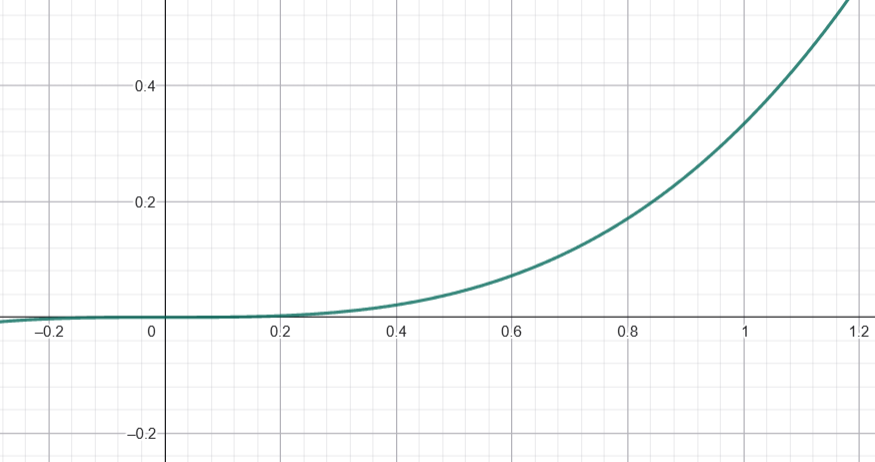
\includegraphics[width=8cm]{5L-1.2-seda.jusjajeva.INF.png}
\end{figure}

$S = 2\pi\integral_0^1\left|\dfrac{1}{3}x^3\right|\sqrt{1 + \left(\left(\dfrac{1}{3}x^3\right)'\right)^2}dx$ \\

$\integral\left|\dfrac{1}{3}x^3\right|\sqrt{1 + \left(\left(\dfrac{1}{3}x^3\right)'\right)^2}dx$ \\

$= \dfrac{1}{3}\integral\left|x^3\right|\sqrt{1 + x^4}dx$ \\

Substitutie: $t = 1 + x^4 \Rightarrow dt = 4x^3dx$ \\

$= \dfrac{1}{12}\integral\sqrt{t}dt$ \\

$= \dfrac{2t^{\tfrac{3}{2}}}{36} + c = \dfrac{(1 + x^4)^{\tfrac{3}{2}}}{18} + c$ \\

$\Rightarrow S = 2\pi\left[\dfrac{(1 + x^4)^{\tfrac{3}{2}}}{18}\right]_0^1 = 2\pi\left(\dfrac{2^{\tfrac{3}{2}}}{18} - \dfrac{1}{18}\right) = \dfrac{2\pi\sqrt{2} - \pi}{9}$ \\



\begin{thebibliography}{999}
%\bibitem{a} Referentie
\end{thebibliography}
\end{document}